\documentclass[11pt]{article}
\usepackage{amsmath,amsthm,amssymb}
\usepackage[margin=1in]{geometry}
\usepackage{stmaryrd}
\usepackage{tikz}
\usetikzlibrary{arrows.meta}
\usepackage[colorlinks=true,linkcolor=blue,citecolor=blue,urlcolor=blue]{hyperref}

\newtheorem{theorem}{Theorem}
\newtheorem{proposition}[theorem]{Proposition}
\newtheorem{corollary}[theorem]{Corollary}
\newtheorem{lemma}[theorem]{Lemma}
\theoremstyle{definition}
\newtheorem{definition}[theorem]{Definition}
\newtheorem{observation}[theorem]{Observation}
\newtheorem{remark}[theorem]{Remark}
\newtheorem{example}[theorem]{Example}

\newcommand{\C}{\mathcal{C}}
\newcommand{\id}{\mathrm{id}}
\newcommand{\Z}{\mathbb{Z}}
\newcommand{\Aut}{\mathrm{Aut}}
\newcommand{\Inn}{\mathrm{Inn}}
\newcommand{\Out}{\mathrm{Out}}
\newcommand{\conj}{\mathrm{conj}}
\newcommand{\gerbe}{\mathfrak{g}}
\newcommand{\Hom}{\mathrm{Hom}}
\newcommand{\coker}{\mathrm{coker}}
\newcommand{\gp}[1]{\langle #1\rangle}
\newcommand{\AUT}{\mathsf{AUT}}
\newcommand{\pizero}{\pi_0}
\newcommand{\pione}{\pi_1}

\title{The $\delta$-commutator lemma is a butterfly\\
\large The automorphism crossed module of the inventory gerbe}
\author{MacBeth\thanks{Kodamai. This is an \emph{expository} companion to the proof note
``The inventory gerbe couples on the torus'' (content commit \texttt{e306ae5}, cited below as
\cite{capstone}); it introduces no new theorem and leaves every grade of that note unchanged.
The present note lives in the author's \texttt{work-in-progress} corpus, content commit
\texttt{0d73790}. Prepared for the Kodamai AI-Mathematician grant (Theory pillar) and for
Neil Ghani's Strathclyde mini-course \emph{Tangent Categories and Containers}, 13--16 October
2026.}\\
\small Kodamai}
\date{13 October 2026}

\begin{document}
\maketitle

\begin{abstract}
The obstruction to reconciling fungible inventory across a supply chain is, following Giraud, a
\emph{tower}: a nonabelian band $\beta\in H^1(N(\C);\Out K)$ in the relabelling group $K=\Aut F$
must vanish before an abelian inventory class is even defined, and on the torus these two stages
turn out to couple through a connecting map given exactly by a commutator of automorphism lifts,
$\delta(\rho)=[[A,B]]$. This note re-reads that result in the language of crossed modules and
butterflies. The whole tower is a \emph{single} crossed module $\partial\colon K\to\Aut K$: its
cokernel $\Out K$ is the band's target, its kernel $Z(K)$ is the inventory coefficient, and its
image $\Inn K$ is the hinge the two Giraud extensions share. A band is a map into the $\pi_0$ of
the associated $2$-group; it lifts strictly iff it extends to a strict morphism of crossed modules,
and it \emph{always} extends to a weak morphism, presented --- following Aldrovandi and Noohi --- by
a \emph{butterfly}. The connecting map is the class of the butterfly's waist extension, and the
commutator $[A,B]$ is literally the commutator of two lifts computed inside the waist group. The
bar--Koszul comparison map that pins the class to this commutator is the butterfly's concrete
cochain model. No result is new; the aim is a picture in which the shared hinge, and the
commutator formula, become inevitable.
\end{abstract}

\section{Introduction}\label{sec:intro}

\paragraph{The result being re-read.} A supply chain is a small category $\C$; inventory is a
datum glued along its morphisms. When local stock charts are comparable only \emph{up to} a
relabelling of states --- up to the automorphism group $K=\Aut F$ of the stock fibre $F$ --- the
gluing datum is an $\Aut F$-gerbe over the nerve $N(\C)$, and the obstruction to a single globally
coherent inventory is, after Giraud \cite{giraud,breen}, not one class but a staged tower. The
relabelling group sits in two group extensions that share their middle term $\Inn K$:
\begin{equation}\label{eq:two-ext}
\text{(I)}\quad 1\to \Inn K\to \Aut K\xrightarrow{\ q\ }\Out K\to 1,
\qquad
\text{(II)}\quad 1\to Z(K)\to K\to \Inn K\to 1.
\end{equation}
The \emph{band} $\beta\in H^1(N(\C);\Out K)$ is read off~(I); it must vanish before the abelian
\emph{inventory class} $[\gerbe]\in H^2(N(\C);Z(K))$ of~(II) is even defined. The companion proof
note \cite{capstone} showed that over the torus $T^2\simeq N(B\Z^2)$ these two stages no longer
clear independently: writing a band as a homomorphism $\rho\colon\Z^2\to\Out K$ (equivalently a
\emph{commuting pair} $\rho(s),\rho(t)$, since $\Z^2$ is abelian), the connecting map from band to
strictification is given exactly by the commutator of any two lifts,
\begin{equation}\label{eq:delta-intro}
\delta(\rho)=[\,[A,B]\,]\in H^2(T^2;\Inn K),\qquad A,B\in\Aut K,\ q(A)=\rho(s),\ q(B)=\rho(t).
\end{equation}
That lemma was proved by a deliberately elementary Schreier-style computation. This note does not
reprove it. It re-reads it.

\paragraph{The gap this note fills.} The proof of~\eqref{eq:delta-intro} is clean but its
\emph{shape} is hidden. Three facts sit side by side in the computation without an evident reason
to be together: that the two Giraud extensions~\eqref{eq:two-ext} share the middle term $\Inn K$;
that the connecting map is a commutator; and that the right coefficient for the strictification
stage is $\Inn K$ while the right coefficient for the inventory stage is $Z(K)$. Why \emph{these}
groups, in \emph{this} arrangement? The elementary proof answers ``because the arithmetic works
out''. We want a reason one can see.

\paragraph{What this note does.} The reason is a single crossed module. Recall that a crossed
module is a homomorphism $\partial\colon C\to G$ with a $G$-action on $C$ satisfying two
compatibilities (\S\ref{sec:xmod}); it is the algebraic incarnation of a $2$-group, and it has two
homotopy groups $\pizero=\coker\partial$ and $\pione=\ker\partial$. The group $K$ carries a
canonical one, the \emph{automorphism crossed module}
\[
\AUT(K):\qquad \partial=\conj\colon K\longrightarrow \Aut K,\qquad k\mapsto c_k\ (\text{conjugation by }k),
\]
and its invariants are exactly the players in~\eqref{eq:two-ext}:
\[
\pizero\AUT(K)=\Out K,\qquad \pione\AUT(K)=Z(K),\qquad \mathrm{im}\,\partial=\Inn K.
\]
The first astonishment (\S\ref{sec:xmod}) is that the two Giraud extensions are \emph{not two
facts}: extension~(I) is the cokernel extension of $\partial$ and~(II) is its kernel extension, so
they are the two edges of one crossed module, necessarily welded at the image $\Inn K$. The shared
hinge is forced.

A band $\rho\colon\Z^2\to\Out K$ is then a map into $\pizero\AUT(K)$ (\S\ref{sec:band}). It lifts
to a strict homomorphism $\Z^2\to\Aut K$ iff it extends to a \emph{strict} morphism of crossed
modules --- and generically it does not. But the honest notion of morphism between crossed modules,
the one that matches maps of the underlying $2$-group stacks, is the \emph{weak} morphism, and
every band extends to one. Following Aldrovandi and Noohi \cite{butterflies}, a weak morphism is
presented by a \emph{butterfly}: a span of groups whose central \emph{waist} is a group extension
(\S\ref{sec:butterfly}). The second astonishment (\S\S\ref{sec:connecting}--\ref{sec:commutator})
is that the proof's pullback extension $E_\rho$ \emph{is} the waist of this butterfly (up to the
centre), so that
\[
\delta(\rho)=\text{the class of the waist extension},
\]
and the commutator $[A,B]$ of~\eqref{eq:delta-intro} is literally the commutator of two lifts
computed \emph{inside the waist group} and pushed to $\Inn K$ by $\partial$. The bar--Koszul
comparison map $\varphi_2(e_{st})=[s\,|\,t]-[t\,|\,s]$ that the proof uses to pin the class is the
concrete cochain shadow of reading this commutator off the waist. Both Giraud stages are instances
of one construction, unified by $\AUT(K)$ (\S\ref{sec:hinge}).

\paragraph{Status.} This is exposition. The underlying lemma, witnesses, and sharp line are proved
and computed in \cite{capstone}; the crossed-module and butterfly translations below are routine
unwindings of definitions, stated as observations, not theorems. The one external input is the
butterfly formalism of \cite{butterflies}, whose bitorsor ancestry is Breen's \cite{breen}; the
classical $H^2\leftrightarrow$ extensions dictionary is Brown \cite{brown} and
Eilenberg--Mac\,Lane \cite{eml}. The intended reader is comfortable with group cohomology and short
exact sequences but has not met $2$-groups or butterflies; \S\ref{sec:xmod} starts from the
definition.

\paragraph{Outline.} Section~\ref{sec:xmod} introduces crossed modules and the automorphism crossed
module, and locates the two Giraud extensions inside it. Section~\ref{sec:band} reads the band as a
map into $\pizero$ and the strict-lifting problem as a strict-morphism-extension problem.
Section~\ref{sec:butterfly} introduces weak morphisms and butterflies, with $\AUT(K)$ as the running
instance. Section~\ref{sec:connecting} identifies the connecting map with the waist class, and
Section~\ref{sec:commutator} identifies the commutator formula with a computation in the waist and
its bar--Koszul shadow. Section~\ref{sec:hinge} returns to the shared hinge and both stages, and
names what the language buys.

\section{The automorphism crossed module}\label{sec:xmod}

\subsection{Crossed modules, gently}

\begin{definition}\label{def:xmod}
A \emph{crossed module} is a group homomorphism $\partial\colon C\to G$ together with a left action
of $G$ on $C$ by automorphisms, written $g\cdot c$, such that
\begin{enumerate}
\item[(E)] $\partial(g\cdot c)=g\,\partial(c)\,g^{-1}$ \quad(\emph{equivariance}), and
\item[(P)] $\partial(c)\cdot c'=c\,c'\,c^{-1}$ \quad(\emph{Peiffer identity}),
\end{enumerate}
for all $g\in G$, $c,c'\in C$. Its \emph{homotopy groups} are
\[
\pizero(\partial)=\coker\partial=G/\mathrm{im}\,\partial,\qquad
\pione(\partial)=\ker\partial.
\]
\end{definition}

A crossed module is the data of a strict $2$-group (equivalently a strict categorical group): $G$
is the group of objects, $G\ltimes C$ the group of arrows, source and target
$s(g)=g$, $t(g,c)=\partial(c)\,g$. The group $\pizero$ is the set of isomorphism classes of objects
--- the ``components'' --- and $\pione$ is the group of automorphisms of the identity object. A
reader who prefers topology may keep in mind the classifying space $B\AUT$, a connected space with
$\pi_1=\pizero$ and $\pi_2=\pione$ and nothing higher; crossed modules are exactly the algebra of
such homotopy $2$-types. We will not need the $2$-group explicitly until \S\ref{sec:band}; for now
$\partial\colon C\to G$ with (E) and (P) is all that is in play.

The Peiffer identity~(P) deserves a word, because it is the condition that makes the two homotopy
groups behave. It forces $\ker\partial$ to be central in $C$ and to be acted on trivially by
$\mathrm{im}\,\partial$: if $\partial(c)=1$ then $c\,c'c^{-1}=\partial(c)\cdot c'=c'$ for all $c'$,
so $\ker\partial\subseteq Z(C)$, and $\pione$ is abelian. This is not a technicality we will skip
past --- it is precisely why the inventory coefficient will come out abelian.

\subsection{The automorphism crossed module}

\begin{proposition}\label{prop:aut-xmod}
Let $K$ be any group. The conjugation map
\[
\partial=\conj\colon K\longrightarrow \Aut K,\qquad k\mapsto c_k\ \ (c_k(x)=kxk^{-1}),
\]
with $\Aut K$ acting on $K$ by evaluation ($\varphi\cdot k:=\varphi(k)$), is a crossed module.
\end{proposition}

\begin{proof}
Both axioms are immediate and worth seeing once. For~(E), $\partial(\varphi\cdot k)=c_{\varphi(k)}$,
while $\varphi\,\partial(k)\,\varphi^{-1}=\varphi\,c_k\,\varphi^{-1}=c_{\varphi(k)}$ since
$\varphi(kxk^{-1})=\varphi(k)\varphi(x)\varphi(k)^{-1}$. For~(P),
$\partial(k)\cdot k'=c_k(k')=kk'k^{-1}$.
\end{proof}

This $\AUT(K)=[\,K\xrightarrow{\conj}\Aut K\,]$ is the \emph{automorphism crossed module} of $K$.
Its invariants read off directly, and they are the whole cast of~\eqref{eq:two-ext}:
\begin{equation}\label{eq:invariants}
\pizero\AUT(K)=\Aut K/\Inn K=\Out K,\qquad
\pione\AUT(K)=\ker(\conj)=Z(K),\qquad
\mathrm{im}\,\partial=\Inn K.
\end{equation}
(That $\ker\conj=Z(K)$ is the statement $c_k=\id\iff k\in Z(K)$; that $\pione$ is abelian is the
Peiffer consequence above, and here it is simply that $Z(K)$ is abelian.)

\subsection{The first astonishment: the tower is one crossed module}

A single homomorphism $\partial\colon C\to G$ breaks into two short exact sequences through its
image. One always has
\[
1\to \ker\partial\to C\to \mathrm{im}\,\partial\to 1
\qquad\text{and}\qquad
1\to \mathrm{im}\,\partial\to G\to\coker\partial\to 1,
\]
glued along $\mathrm{im}\,\partial$. For $\partial=\conj\colon K\to\Aut K$ these are, by
\eqref{eq:invariants}, \emph{exactly} the two Giraud extensions:
\begin{equation}\label{eq:edges}
\underbrace{1\to Z(K)\to K\to \Inn K\to 1}_{\text{(II): kernel extension}}
\qquad\text{and}\qquad
\underbrace{1\to \Inn K\to \Aut K\xrightarrow{q}\Out K\to 1}_{\text{(I): cokernel extension}}.
\end{equation}

\begin{observation}\label{obs:hinge}
The two extensions~\eqref{eq:two-ext} of the inventory gerbe are the kernel extension and the
cokernel extension of the single crossed module $\AUT(K)$. They share the hinge $\Inn K$ because
$\Inn K=\mathrm{im}\,\partial$ is at once the cokernel of $\conj\colon K\to\Inn K$ (the quotient in
(II)) and the kernel of $q\colon\Aut K\to\Out K$ (the normal subgroup in (I)). No coincidence is
needed: $\mathrm{im}\,\partial$ is the unique group through which any homomorphism factors.
\end{observation}

\begin{center}
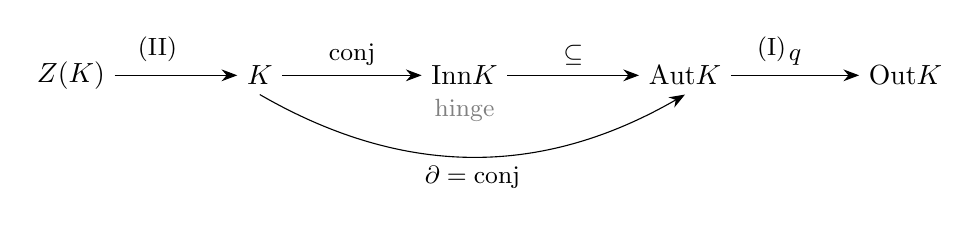
\begin{tikzpicture}[>={Stealth[length=2mm]},node distance=16mm]
\node (Z) at (0,0) {$Z(K)$};
\node (K) at (2.4,0) {$K$};
\node (Inn) at (5.0,0) {$\Inn K$};
\node (Aut) at (7.8,0) {$\Aut K$};
\node (Out) at (10.6,0) {$\Out K$};
\draw[->] (Z) -- (K);
\draw[->] (K) -- node[above,font=\small] {$\conj$} (Inn);
\draw[->] (Inn) -- node[above,font=\small] {$\subseteq$} (Aut);
\draw[->] (Aut) -- node[above,font=\small] {$q$} (Out);
\draw[->] (K.south) to[out=-30,in=-150] node[below,font=\small] {$\partial=\conj$} (Aut.south);
\node[font=\small] at (1.1,0.33) {(II)};
\node[font=\small] at (8.9,0.33) {(I)};
\node[font=\small,gray] at (5.0,-0.45) {hinge};
\end{tikzpicture}
\end{center}

\noindent The crossed module $\partial\colon K\to\Aut K$ is the lower arc; it factors as the
surjection $K\twoheadrightarrow\Inn K$ (giving~(II) on the left) followed by the inclusion
$\Inn K\hookrightarrow\Aut K$ (giving~(I) on the right). Reading the diagram once makes the staged
structure of the gerbe obstruction visible as a single object rather than a pair of accidents: the
band lives on the right edge, the inventory class on the left edge, and the kernel $Z(K)$ and
cokernel $\Out K$ are the two homotopy groups of the $2$-group that the whole thing is.

\section{The band as a map into \texorpdfstring{$\pizero$}{pi0}}\label{sec:band}

\subsection{Bands}

Fix throughout a base $T^2\simeq N(B\Z^2)$: two commuting reversible operations. A band on $T^2$ is
a class in $H^1(T^2;\Out K)$, which for the free base $B\Z^2$ is exactly a homomorphism
\[
\rho\colon\Z^2\longrightarrow\Out K,
\]
and, because $\Z^2=\gp{s,t\mid [s,t]}$ is abelian, exactly a \emph{commuting pair}
$\rho(s),\rho(t)\in\Out K$. Under~\eqref{eq:invariants}, $\Out K=\pizero\AUT(K)$: a band is a map
from $\Z^2$ \emph{into the components of the automorphism $2$-group}. The strictification question
of the Giraud tower --- can the band be realised by an honest, inner-free transport? --- is the
question of \emph{lifting $\rho$ through the $2$-group}.

\subsection{Strict morphisms are too rigid}

The flat-footed way to lift $\rho$ is to ask for a homomorphism $\tilde\rho\colon\Z^2\to\Aut K$ with
$q\circ\tilde\rho=\rho$: a \emph{strict lift}. In crossed-module terms this is a strict morphism.
Regard $\Z^2$ as the \emph{discrete} crossed module $[\,1\to\Z^2\,]$ --- trivial in degree one, so
$\pizero=\Z^2$ and $\pione=0$. A strict morphism $[\,1\to\Z^2\,]\to[\,K\to\Aut K\,]$ is, by
definition, a pair of homomorphisms (one in each degree) commuting with the two $\partial$'s and the
actions; in degree one the only map out of the trivial group is trivial, so a strict morphism is
\emph{nothing but} a homomorphism $\Z^2\to\Aut K$ lifting $\rho$ on $\pizero$.

\begin{observation}\label{obs:strict}
A strict morphism of crossed modules $[\,1\to\Z^2\,]\to\AUT(K)$ inducing $\rho$ on $\pizero$ is the
same datum as a strict lift $\tilde\rho\colon\Z^2\to\Aut K$ of the band, i.e.\ a pair of
\emph{commuting} lifts $A=\tilde\rho(s)$, $B=\tilde\rho(t)$.
\end{observation}

And here is the difficulty the whole subject is about: strict lifts usually do not exist. Two outer
classes may commute in $\Out K$ while \emph{no} choice of representatives commutes in $\Aut K$. The
band $\rho$ remembers only the components; whether it lifts remembers the $2$-group. The strict
morphism is the wrong tool because it demands the lift on the nose. The next section supplies the
right tool, which demands only that the lift exist \emph{up to coherent inner slack} --- and then
measures the slack.

\section{Weak morphisms and butterflies}\label{sec:butterfly}

\subsection{Why weak morphisms}

Crossed modules present $2$-groups, and the honest morphisms of $2$-groups --- the ones that
correspond to maps of classifying spaces, or of the associated stacks --- are \emph{weak}: they
need respect the structure only up to coherent isomorphism. Inverting the weak equivalences of
crossed modules (the morphisms that are isomorphisms on both $\pizero$ and $\pione$) turns the
strict morphisms into a larger class of fractions. Aldrovandi and Noohi \cite{butterflies} gave
these fractions a concrete, diagram-level description --- the \emph{butterfly} --- so that one never
has to leave the category of groups to compute with weak morphisms. We state the definition in the
generality we use and immediately specialise.

\begin{definition}[Aldrovandi--Noohi \cite{butterflies}]\label{def:butterfly}
Let $[\,C_1\xrightarrow{\partial_1}G_1\,]$ and $[\,C_2\xrightarrow{\partial_2}G_2\,]$ be crossed
modules. A \emph{butterfly} between them is a group $E$ together with four homomorphisms
\[
C_1\xrightarrow{\ \kappa\ }E\xleftarrow{\ \iota\ }C_2,\qquad
G_1\xleftarrow{\ p\ }E\xrightarrow{\ q\ }G_2,
\]
arranged as the two diagonals of
\begin{center}
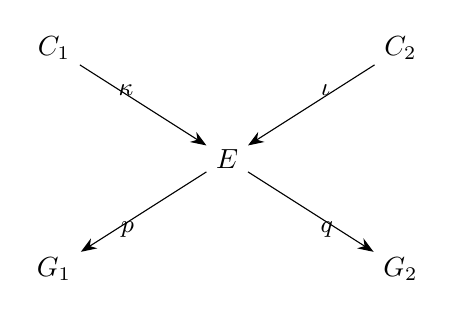
\begin{tikzpicture}[>={Stealth[length=2mm]},scale=1.0]
\node (C1) at (-2.2,1.4) {$C_1$};
\node (C2) at (2.2,1.4) {$C_2$};
\node (E) at (0,0) {$E$};
\node (G1) at (-2.2,-1.4) {$G_1$};
\node (G2) at (2.2,-1.4) {$G_2$};
\draw[->] (C1) -- node[above left,font=\small] {$\kappa$} (E);
\draw[->] (C2) -- node[above right,font=\small] {$\iota$} (E);
\draw[->] (E) -- node[below left,font=\small] {$p$} (G1);
\draw[->] (E) -- node[below right,font=\small] {$q$} (G2);
\end{tikzpicture}
\end{center}
such that
\begin{enumerate}
\item[(B1)] the NE--SW diagonal $1\to C_2\xrightarrow{\iota}E\xrightarrow{p}G_1\to1$ is
\emph{short exact};
\item[(B2)] the NW--SE diagonal $C_1\xrightarrow{\kappa}E\xrightarrow{q}G_2$ is a \emph{complex}
($q\kappa=1$);
\item[(B3)] $p\,\kappa=\partial_1$ and $q\,\iota=\partial_2$; and
\item[(B4)] $\kappa$ and $\iota$ are equivariant for the conjugation action of $E$ on itself
(pulled back from the $G_i$-actions along $p$ and $q$).
\end{enumerate}
A butterfly represents a weak morphism $[\,C_1\to G_1\,]\to[\,C_2\to G_2\,]$, the exact leg~(B1)
being the weak equivalence one inverts: the span is $G_1\xleftarrow{p}E\xrightarrow{q}G_2$ with
$p$ invertible up to $C_2$.
\end{definition}

The picture earns its name: the two top wings are the degree-one groups mapping \emph{into} the
central body $E$, the two bottom wings are the degree-zero groups $E$ projects \emph{onto}, and the
whole is pinched at the waist $E$. The essential content, for us, is axiom~(B1): the body $E$ is an
\emph{extension} --- of the source's degree-zero group by the target's degree-one group. This is
where a cohomology class will live.

\subsection{The running butterfly}

Specialise to source $[\,1\to\Z^2\,]$ and target $\AUT(K)=[\,K\xrightarrow{\conj}\Aut K\,]$. Then
$C_1=1$, $G_1=\Z^2$, $C_2=K$, $G_2=\Aut K$, and a butterfly is a group $E$ with
\begin{center}
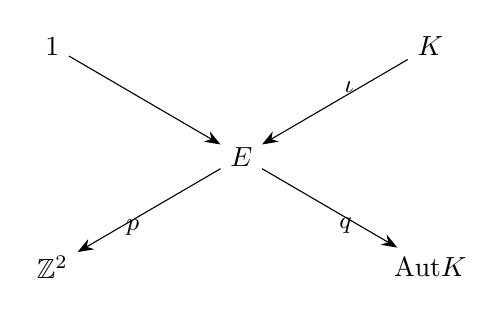
\begin{tikzpicture}[>={Stealth[length=2mm]}]
\node (C1) at (-2.4,1.4) {$1$};
\node (C2) at (2.4,1.4) {$K$};
\node (E) at (0,0) {$E$};
\node (G1) at (-2.4,-1.4) {$\Z^2$};
\node (G2) at (2.4,-1.4) {$\Aut K$};
\draw[->] (C1) -- (E);
\draw[->] (C2) -- node[above right,font=\small] {$\iota$} (E);
\draw[->] (E) -- node[below left,font=\small] {$p$} (G1);
\draw[->] (E) -- node[below right,font=\small] {$q$} (G2);
\end{tikzpicture}
\end{center}
whose only nontrivial data are the \emph{waist extension} and the map $q$:
\begin{equation}\label{eq:waist}
\text{(B1)}\quad 1\to K\xrightarrow{\ \iota\ }E\xrightarrow{\ p\ }\Z^2\to1,
\qquad
\text{(B3)}\quad q\colon E\to\Aut K,\ \ q\circ\iota=\conj.
\end{equation}
Unwound: a butterfly here is a group $E$ extending $\Z^2$ by the whole of $K$, together with a
homomorphism $q\colon E\to\Aut K$ that restricts on the normal copy of $K$ to conjugation. The
weak morphism it carries induces on $\pizero$ the map $\Z^2\to\Out K$ sending $\gamma\in\Z^2$ to
the class of $q(\hat\gamma)$, where $\hat\gamma\in E$ is any element with $p(\hat\gamma)=\gamma$
(well-defined modulo $q(K)=\Inn K$). That induced map is the band:

\begin{observation}\label{obs:butterfly-band}
A butterfly $E$ as in~\eqref{eq:waist} induces the band $\rho\colon\Z^2\to\Out K$ on $\pizero$. A
homomorphic section $\tilde\rho\colon\Z^2\to E$ of the waist (if one exists) yields a strict lift
$q\tilde\rho\colon\Z^2\to\Aut K$ of $\rho$ --- a pair of commuting lifts, as in
Observation~\ref{obs:strict} --- so that the weak morphism carried by $E$ becomes isomorphic to a
strict morphism.
\end{observation}

So the passage from ``strict lift'' to ``butterfly'' is the passage from ``the band lifts to a
homomorphism'' to ``the band lifts only into an \emph{extension}''. The obstruction to going back
is a cohomology class, and that class is the connecting map, measured on the quotient $E_\rho$ of
the waist (\S\ref{sec:connecting}).

\section{The connecting map is the waist}\label{sec:connecting}

The proof note \cite{capstone} forms, for a band $\rho$, the pullback extension
\[
E_\rho:=\Aut K\times_{\Out K}\Z^2=\{(a,\gamma)\in\Aut K\times\Z^2:q(a)=\rho(\gamma)\},
\qquad 1\to\Inn K\to E_\rho\xrightarrow{\ \bar p\ }\Z^2\to1,
\]
and \emph{defines} $\delta(\rho):=[E_\rho]\in H^2(T^2;\Inn K)$. This is the waist of the running
butterfly, pushed down past the centre.

\begin{proposition}\label{prop:waist-is-Erho}
Let $E$ be a butterfly as in~\eqref{eq:waist} inducing $\rho$. The map
$(q,p)\colon E\to\Aut K\times\Z^2$ lands in $E_\rho$ and induces an isomorphism
\[
E/\,\iota(Z(K))\ \xrightarrow{\ \sim\ }\ E_\rho,
\]
carrying the waist extension~\eqref{eq:waist} of $\Z^2$ by $K$ onto the pullback extension of
$\Z^2$ by $\Inn K$ along the quotient $K\twoheadrightarrow\Inn K$. Consequently
$\delta(\rho)=[E_\rho]$ is the image of the waist class under $K\twoheadrightarrow\Inn K$.
\end{proposition}

\begin{proof}
For $e\in E$ one has $q(e)\in\Aut K$ and $p(e)\in\Z^2$ with
$q(e)\bmod\Inn K=\rho(p(e))$ by Observation~\ref{obs:butterfly-band}; hence
$(q(e),p(e))\in E_\rho$, so $(q,p)$ is a homomorphism $E\to E_\rho$. It is surjective because $p$ is
surjective and $q|_K=\conj$ surjects $K$ onto the fibre $\Inn K$ of $E_\rho$ over $0$. Its kernel is
$\{e:p(e)=0,\ q(e)=\id\}$; by~(B1), $p(e)=0$ means $e=\iota(k)$ for a unique $k\in K$, and then
$q(e)=\conj(k)=\id$ means $k\in\ker\conj=Z(K)$. So $\ker(q,p)=\iota(Z(K))$, a normal subgroup
(being a kernel), and the stated isomorphism is the first isomorphism theorem. The extension statement is the commuting square
\[
\begin{array}{ccc}
K & \longrightarrow & E\\
\big\downarrow && \big\downarrow\\
\Inn K & \longrightarrow & E_\rho
\end{array}
\]
with vertical maps the quotients by $Z(K)$, exhibiting $E_\rho$ as the pushout of~\eqref{eq:waist}
along $K\twoheadrightarrow\Inn K$.
\end{proof}

\begin{observation}\label{obs:split-dictionary}
Under Proposition~\ref{prop:waist-is-Erho}, the three vanishing conditions line up:
\[
\begin{aligned}
\delta(\rho)=0
\ &\overset{\text{\cite[IV.3]{brown}}}{\iff}\ E_\rho\text{ splits}
\ \iff\ \rho\text{ has a strict lift}\\
&\iff\ \text{the weak morphism carried by the butterfly is isomorphic to a strict one}.
\end{aligned}
\]
\end{observation}

That is the whole conceptual content of the connecting map, now visible: $\delta(\rho)$ is the
obstruction to the waist of the butterfly being split, equivalently to the band's weak lift being
strictifiable. The proof note establishes the equivalence $\delta(\rho)=0\iff$ (commuting lifts)
by the classical extension dictionary \cite{brown,eml}; here the same equivalence is read off the
butterfly. What remains --- the \emph{value} of the class when it does not vanish --- is a
commutator, and it too lives in the waist.

\section{The commutator is a commutator in the waist}\label{sec:commutator}

\subsection{The commutator lives upstairs}

Choose lifts of the $\Z^2$-generators into the waist: $\hat s,\hat t\in E$ with $p(\hat s)=s$,
$p(\hat t)=t$. Their images $A:=q(\hat s)$, $B:=q(\hat t)\in\Aut K$ are lifts of
$\rho(s),\rho(t)$ in the sense of~\eqref{eq:delta-intro}. Because $s$ and $t$ commute in $\Z^2$,
the commutator $[\hat s,\hat t]$ lies in $\ker p=\iota(K)$, so it \emph{is} an element of $K$:
\begin{equation}\label{eq:comm-upstairs}
[\hat s,\hat t]=\iota(w_0),\qquad w_0\in K.
\end{equation}
Apply $q$ and use $q\iota=\conj$:
\begin{equation}\label{eq:comm-down}
[A,B]=[q(\hat s),q(\hat t)]=q([\hat s,\hat t])=q(\iota(w_0))=\conj(w_0)=c_{w_0}\in\Inn K.
\end{equation}

\begin{observation}\label{obs:commutator}
The $\Inn K$-valued commutator $w=[A,B]$ of~\eqref{eq:delta-intro} is the image under
$\partial=\conj$ of a genuine $K$-valued commutator $w_0=[\hat s,\hat t]$ measured \emph{inside the
butterfly's waist}. The outer-level ``$[A,B]$ fails to vanish'' is the shadow of the honest group
commutator of two chosen lifts failing to be central.
\end{observation}

This is the cleanest way to see why a commutator appears at all. The band records a pair of
commuting \emph{outer} classes; lifting it into the waist chooses honest group elements
$\hat s,\hat t$; they need not commute, and \emph{their commutator is the whole obstruction},
because it is exactly the element of $K\subseteq E$ one picks up on traversing the torus's defining
loop $sts^{-1}t^{-1}$.

\subsection{The bar--Koszul shadow}

To turn~\eqref{eq:comm-down} into a cohomology class in the correct coordinates, the proof note
reads the waist extension through a factor set and compares resolutions. We recall the mechanism
only to the depth that shows it is the cochain shadow of Observation~\ref{obs:commutator}; the
computation itself is \cite[\S3]{capstone}.

Over $R=\Z[\Z^2]=\Z[s^{\pm1},t^{\pm1}]$ there are two free resolutions of the trivial module $\Z$:
the small \emph{Koszul} resolution, whose top differential encodes the single torus relator and
which computes
\[
H^2(T^2;M)=M\big/\big((\sigma-1)M+(\tau-1)M\big)=M_{\Z^2}\qquad(\sigma,\tau=\text{the }\Z^2\text{-action}),
\]
and the large \emph{bar} resolution, in which a factor set of an extension is literally a
$2$-cocycle $f(g,h)$. The unique-up-to-homotopy comparison map $\varphi\colon K_\bullet\to B_\bullet$
sends the fundamental $2$-cell to the antisymmetric expression
\begin{equation}\label{eq:phi2}
\varphi_2(e_{st})=[s\,|\,t]-[t\,|\,s],
\end{equation}
so that evaluation of any bar $2$-cocycle $f$ on the generator of $H^2(T^2;M)$ is
$\varphi^*[f]=[\,f(s,t)-f(t,s)\,]\in M_{\Z^2}$. Expression~\eqref{eq:phi2} is the algebraic shadow
of the loop $sts^{-1}t^{-1}$: the two orderings of the cell, with opposite signs.

Now take $M=\Inn K$ and the factor set of the waist extension $E_\rho$ for the section
$u(s^it^j)=\hat s^{\,i}\hat t^{\,j}$ (the same lifts as above, pushed to $\Inn K$). One computes,
using $st=ts$,
\[
f(s,t)=u(s)u(t)u(st)^{-1}=1,\qquad
f(t,s)=u(t)u(s)u(ts)^{-1}=\hat t\hat s(\hat s\hat t)^{-1}=[\hat s,\hat t]^{-1}=w^{-1}
\]
in $\Inn K$. Hence, by~\eqref{eq:phi2},
\begin{equation}\label{eq:delta-value}
\delta(\rho)=\varphi^*[f]=[\,f(s,t)-f(t,s)\,]=[\,0-(-w)\,]=[\,w\,]=[\,[A,B]\,]\in \Inn K_{\,\Z^2}.
\end{equation}
The antisymmetric $[s|t]-[t|s]$ of~\eqref{eq:phi2} is nothing but the two orderings $f(s,t)$ and
$f(t,s)$, whose quotient is the commutator; the comparison map is the bookkeeping that makes
``evaluate on the torus $2$-cell'' mean ``take the commutator of the lifts in the waist''. The
class $[w]$ is independent of the lifts because changing $\hat s,\hat t$ by elements of
$\ker p=K$ changes $w$ by a coboundary (the lift-independence computation of \cite{capstone}); in
the butterfly this is the statement that different section-choices give isomorphic waist extensions.

\begin{remark}[trivial action and the clean slogan]\label{rem:trivial}
When $\sigma=\tau=\id$ --- the case of every explicit witness in \cite{capstone}, where the lifts
act trivially on $\Inn K$ --- the coboundaries vanish, $\Inn K_{\Z^2}=\Inn K$, and
\eqref{eq:delta-value} reduces to the bare slogan $\delta(\rho)=[A,B]\neq0$. The coinvariant
quotient $M_{\Z^2}$ is the correction the general lemma carries for a nontrivial action; it is the
$\pizero$-coinvariants of $\pione$-with-a-twist, exactly what a $2$-group hands to $H^2$.
\end{remark}

\section{The shared hinge, and both stages at once}\label{sec:hinge}

We treated the band-to-strictification stage, extension~(I), with the butterfly into
$\AUT(K)=[\,K\to\Aut K\,]$. The inventory stage, extension~(II), is the same picture one edge to the
left. The general lemma of \cite{capstone} applies to \emph{any} abelian-kernel extension
$1\to M\to \mathcal{E}\to Q\to1$ and band $\Z^2\to Q$; the two Giraud stages are its two instances,
\[
\text{(I)}\quad(\mathcal{E},Q,M)=(\Aut K,\Out K,\Inn K),\qquad
\text{(II)}\quad(\mathcal{E},Q,M)=(K,\Inn K,Z(K)),
\]
and both are edges of the one crossed module $\AUT(K)$ by Observation~\ref{obs:hinge}. The kernel
edge~(II) has coefficient $Z(K)=\pione$, abelian for \emph{every} $K$ by the Peiffer identity; the
cokernel edge~(I) has coefficient $\Inn K$, abelian exactly when $K$ has nilpotency class $\le2$
--- the standing hypothesis of \cite{capstone}, now identified as the condition that the
\emph{image} of $\partial$, not merely its kernel, be abelian.

\begin{observation}\label{obs:both-stages}
The hinge $\Inn K$ carries both stages: as the \emph{quotient} in~(II) it is the target of the
inventory band, and as the \emph{kernel} in~(I) it is the coefficient of the strictification class.
The coupling of the two stages on $T^2$ --- a nonzero band forcing a nonzero class --- is therefore
a statement about a single crossed module failing to be ``split on both edges'' over $\Z^2$, and
the common mechanism, a commutator of lifts in a waist, is the same on each edge.
\end{observation}

\paragraph{What the language buys.} The butterfly reformulation proves nothing the Schreier
computation did not, but it makes three things structural rather than incidental. First, the shared
hinge is forced (Observation~\ref{obs:hinge}): one cannot have the two Giraud extensions without
their sharing $\Inn K$, because they are the two factorisation-edges of one map. Second, the
commutator is forced (Observation~\ref{obs:commutator}): the obstruction is a commutator because it
is \emph{the} element of the fibre one collects traversing the torus relator in the waist group,
not a feature of the particular group $K$. Third, the coefficients are forced: $\pione=Z(K)$ is
abelian by Peiffer, and the class-$\le2$ hypothesis is exactly $\mathrm{im}\,\partial$ abelian ---
the hypothesis is read off the crossed module, not imposed by hand.

\paragraph{What it suggests.} Butterflies compose, and composition of butterflies is composition of
weak morphisms of $2$-groups \cite{butterflies}. Two welds along a reconvergent logistics network
compose as a Zappa--Sz\'ep-type overlay; whether that composite weld's obstruction is the composite
of the butterflies' waist classes is a clean question the present language poses but does not
settle, and it is the natural next node. A second is the passage beyond class $\le2$: dropping that
hypothesis makes $\mathrm{im}\,\partial=\Inn K$ nonabelian, so the cokernel edge~(I) leaves the
abelian-kernel world and the butterfly's waist class becomes a genuinely nonabelian datum --- the
Breen bitorsor register \cite{breen} that the Aldrovandi--Noohi formalism was built to carry
\cite{butterflies}. Neither is claimed here; both are \emph{open}, and the butterfly picture is
what makes them precise.

\begin{thebibliography}{9}
\bibitem{butterflies} E.~Aldrovandi and B.~Noohi, \emph{Butterflies~I: Morphisms of $2$-group
stacks}, Advances in Mathematics \textbf{221} (2009), 687--773; arXiv:0808.3627.
\bibitem{breen} L.~Breen, \emph{Bitorseurs et cohomologie non ab\'elienne}, in: The Grothendieck
Festschrift, Vol.~I, Progr. Math.\ 86, Birkh\"auser, 1990, pp.~401--476.
\bibitem{brown} K.~S.~Brown, \emph{Cohomology of Groups}, Graduate Texts in Mathematics 87,
Springer, 1982 (Chapter~IV).
\bibitem{eml} S.~Eilenberg and S.~Mac\,Lane, \emph{Cohomology theory in abstract groups.~II.
Group extensions with a non-Abelian kernel}, Ann.\ of Math.\ (2) \textbf{48} (1947), 326--341.
\bibitem{giraud} J.~Giraud, \emph{Cohomologie non ab\'elienne}, Grundlehren der mathematischen
Wissenschaften 179, Springer, 1971 (Chapters III--IV).
\bibitem{capstone} MacBeth, \emph{The inventory gerbe couples on the torus}, Kodamai
work-in-progress note, content commit \texttt{e306ae5}, 12 October 2026.
\end{thebibliography}

\end{document}
